\title{Оценка гетерогенности эффектов}
\author[Георгий Калашнов, Ольга Сучкова]{Георгий Калашнов, Ольга Сучкова}
\date{\today}

\begin{document}

\begin{frame}
  \titlepage
  
\end{frame}


\begin{frame}{План на сегодня} 
\tableofcontents
\end{frame}

\section{Инструментальные переменные: пробуем на данных}

\begin{frame}{Президентские выборы во Франции 2012 \parencite{pons2018will}}
\begin{columns}
\begin{column}{0.5\textwidth}
    
   \begin{center}
   Франсуа Олланд
   \vskip1em
     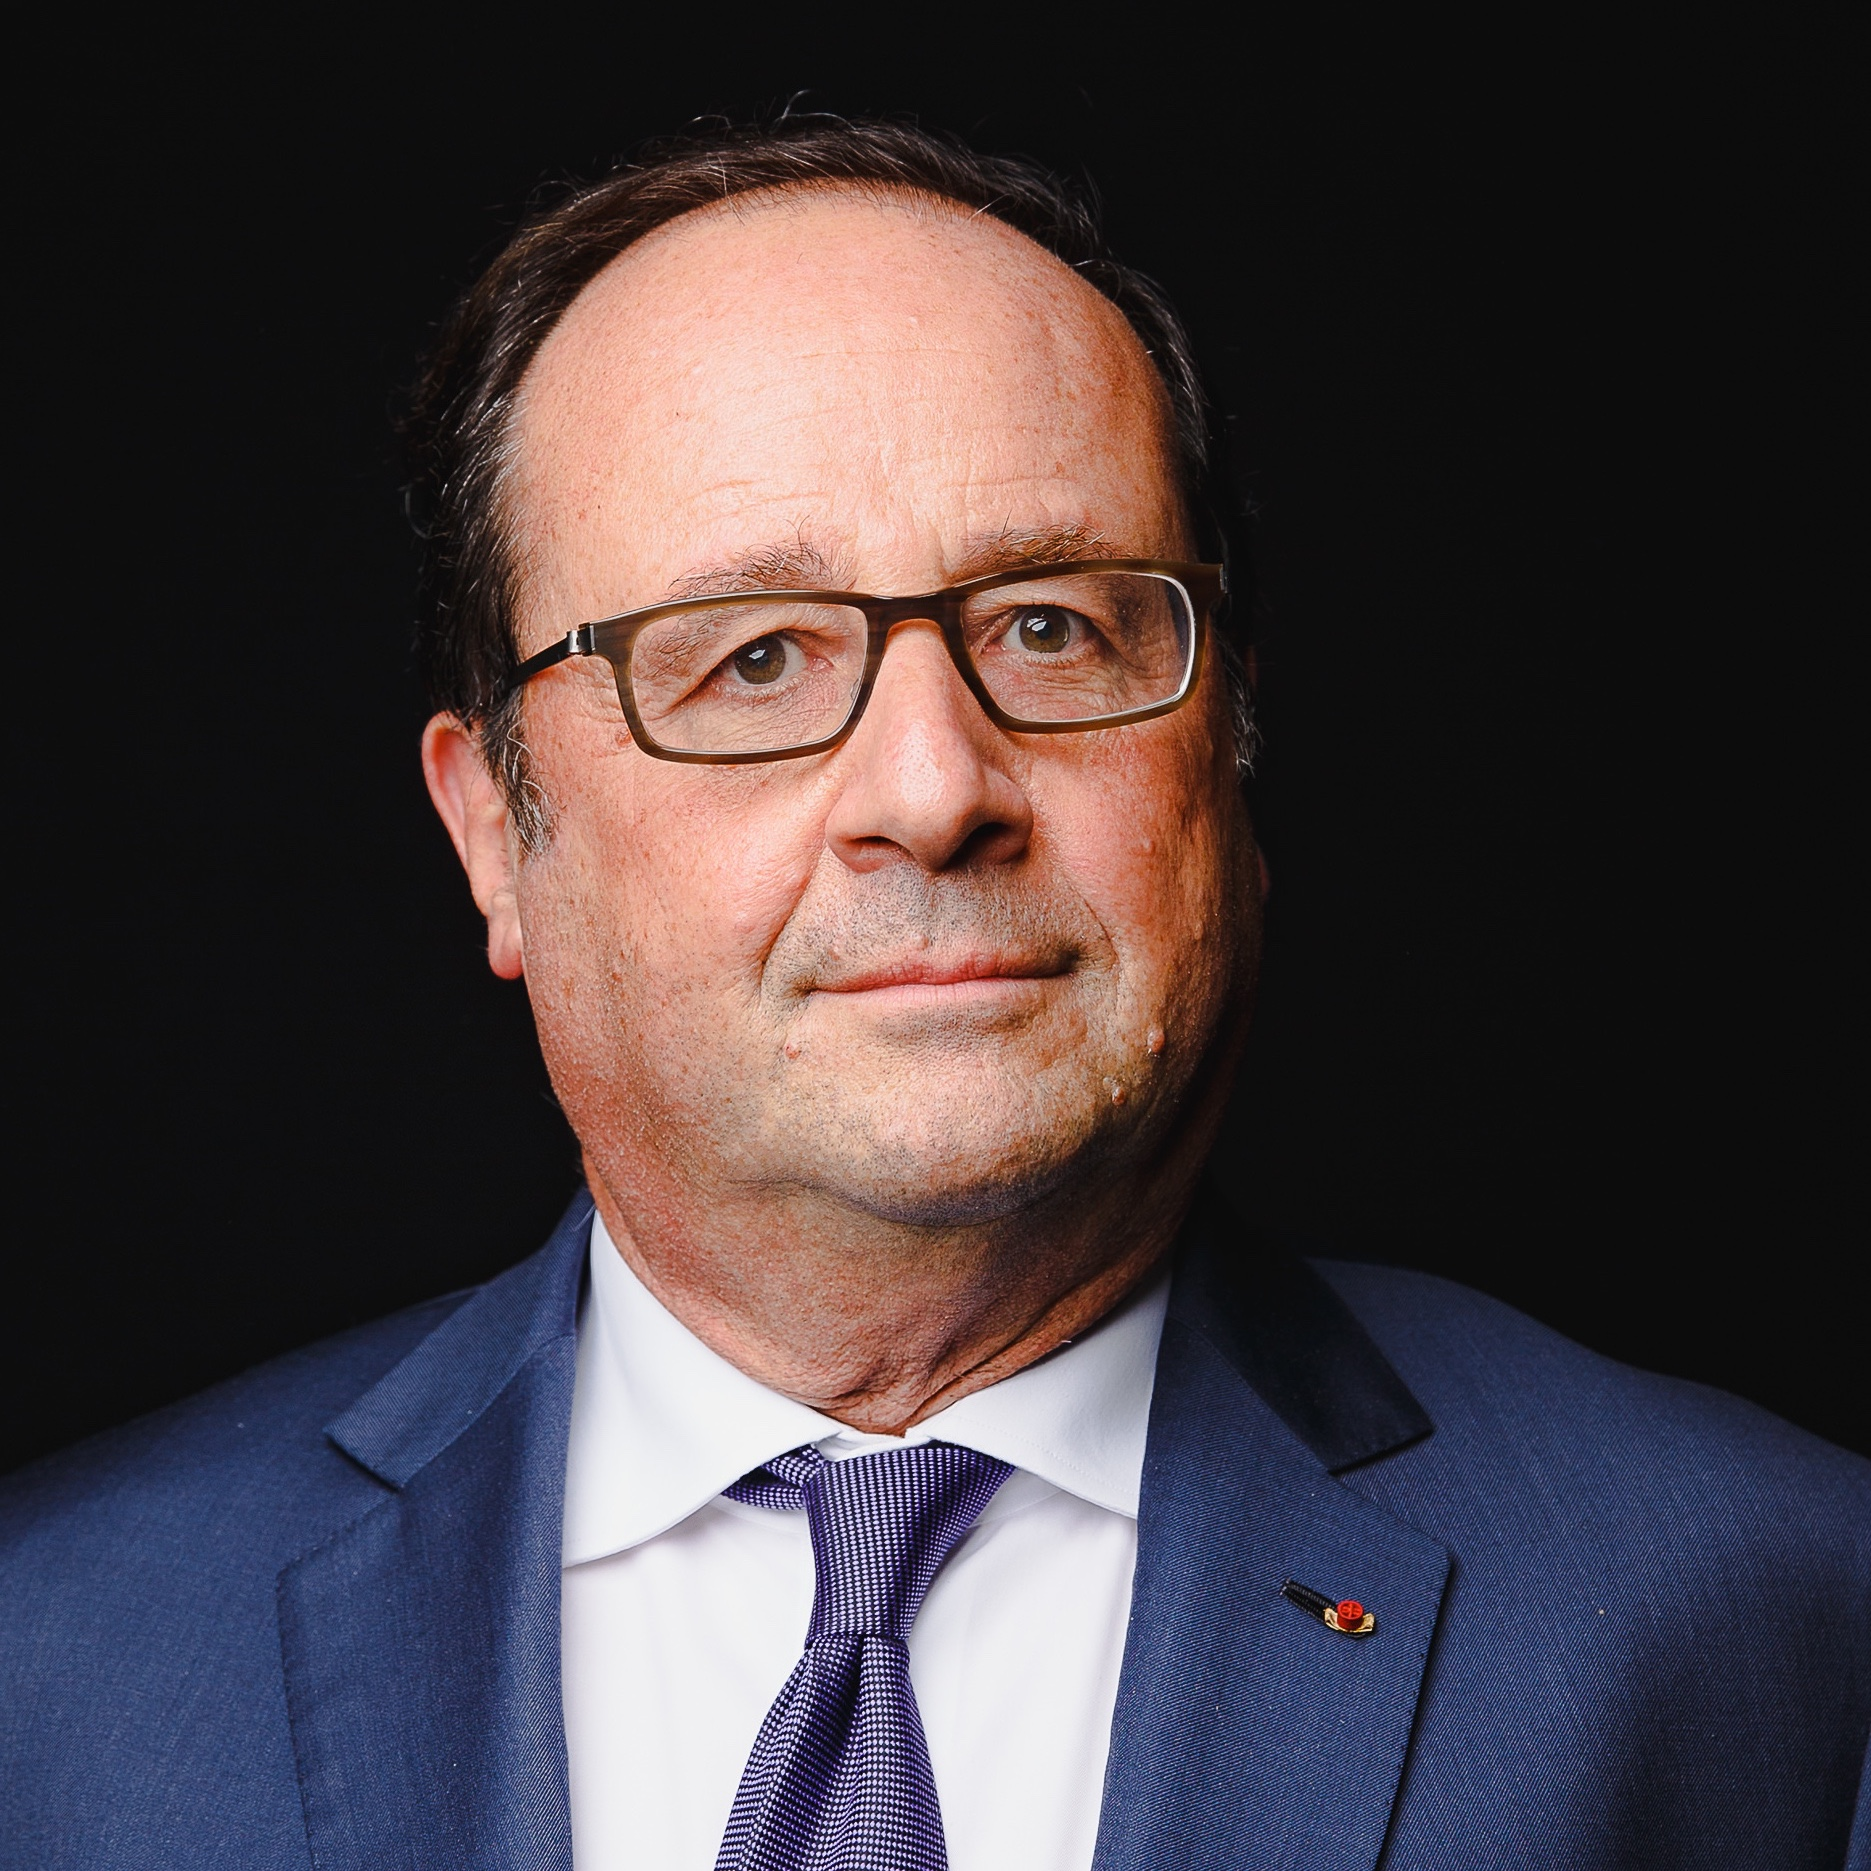
\includegraphics[width=0.8\textwidth]{Lecture_Sources/Images/hollande.jpg}
     \vskip1em
     
\includegraphics[width=0.8\textwidth]{Lecture_Sources/Images/hollande_effect.png}
     \end{center}
\end{column}
\begin{column}{0.5\textwidth} 
    
    \begin{center}
    Николя Саркози
    \vskip1em
     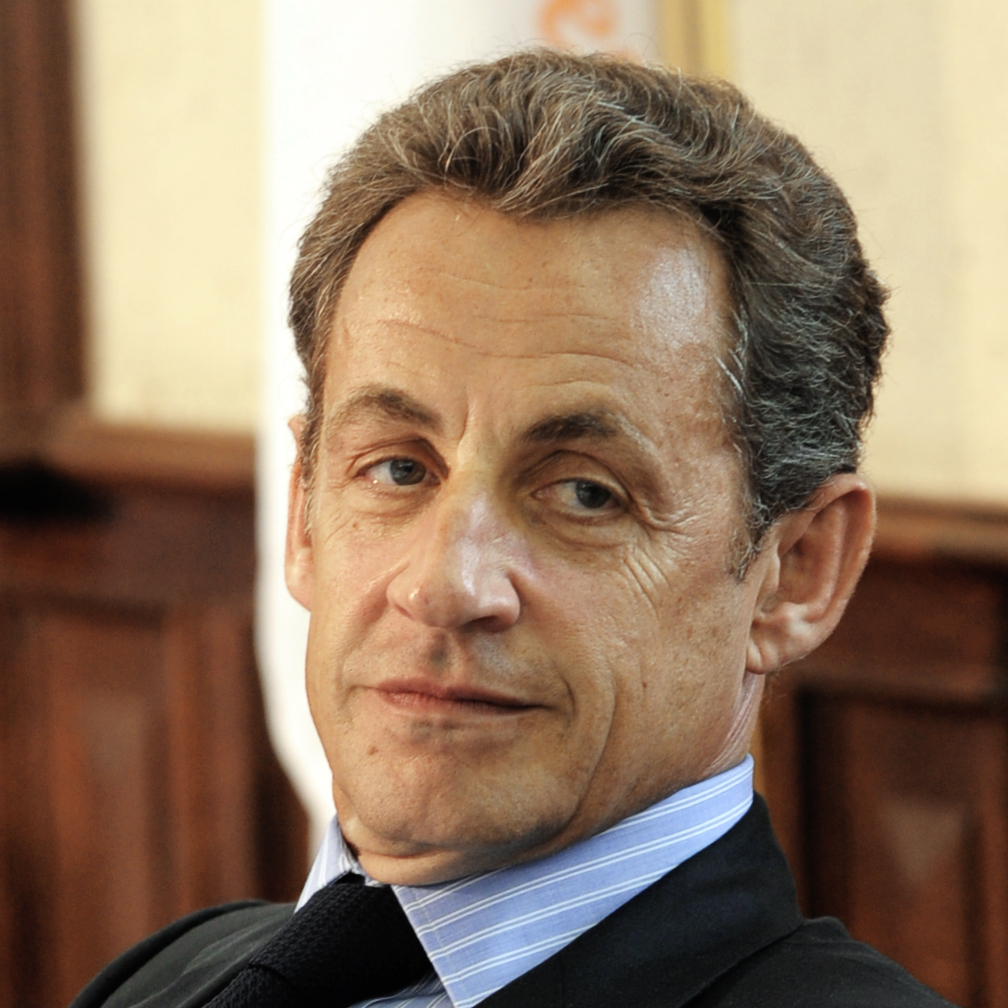
\includegraphics[width=0.8\textwidth]{Lecture_Sources/Images/sarkozy.jpg}
     \vskip1em
     
\includegraphics[width=0.8\textwidth]{Lecture_Sources/Images/sarkozy_votes.png}
     \end{center}
\end{column}
\end{columns}
Эффект от агитации в 0.5 процентных пункта. 
\end{frame}


\begin{frame}{Президентские выборы во Франции 2012 \parencite{pons2018will}}

\begin{enumerate}
    \item Не все агитаторы исполняли агитационные предписания.
    \item Какой эффект мы получаем простым сравнением тестовой и контрольной группы?
\end{enumerate}

\begin{enumerate}
    \item Мы имеем дело с односторонним или двусторонним неповиновением treatment?
    \item Давайте попробуем оценить IV (двумя способами)
\end{enumerate}

\end{frame}



\section{Гетерогенность эффектов}

\begin{frame}{Оценка гетерогенности как таковой}
Тема очень сложная, поэтому в рамках МФК мы ее очертим только в общих чертах

Что такое гетерогенность еще раз

$$
\tau(x) = \mathbb{E}(Y|X=x)
$$

Зачем мы можем хотеть оценить гетерогенность

\begin{enumerate}
    \item Чтобы установить ее наличие или отсутствие
    \item Чтобы понять масштаб гетерогенности
    \item для рекомендаций (policy advice)
    \begin{enumerate}
        \item Оценка кредитоспособности
        \item Таргетирование грантов
        \item Таргетирование маркетинга
    \end{enumerate}
\end{enumerate}
\end{frame}

\begin{frame}{Пример: таргетирование маркетинга}
\begin{figure}
    \centering
    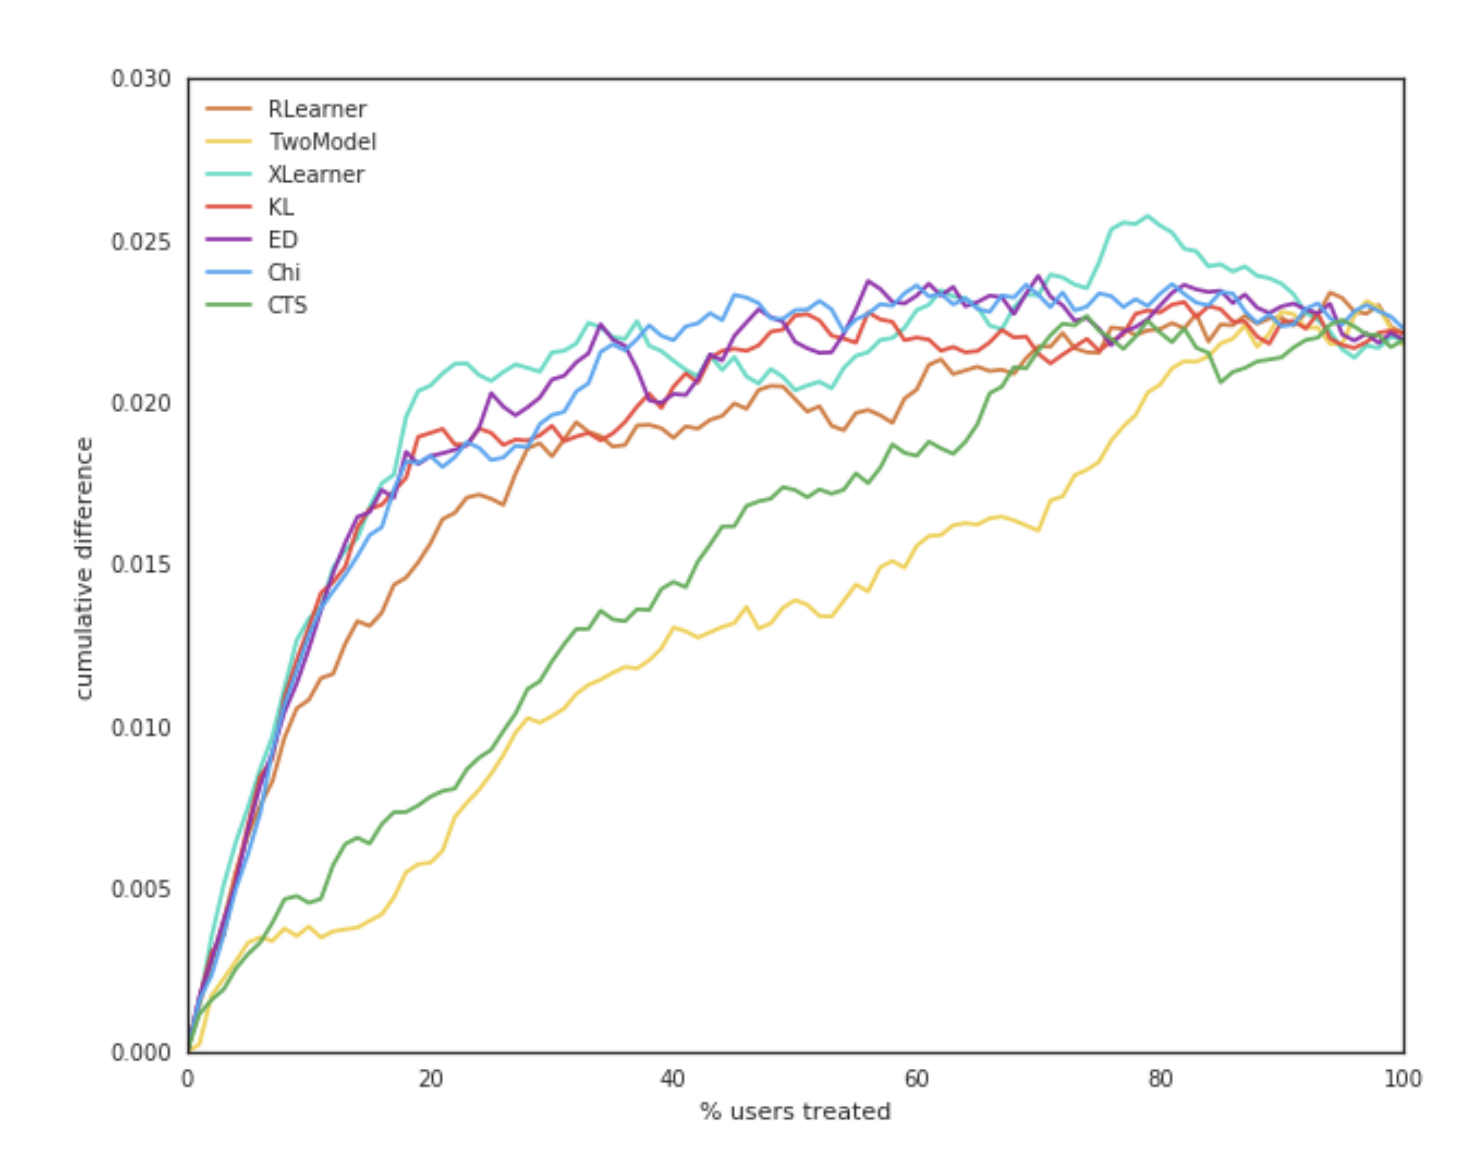
\includegraphics[width=\textwidth]{uplift_tmp.png}
\end{figure}
\end{frame}

\begin{frame}{Пример: таргетирование грантов}
\begin{figure}
    \centering
    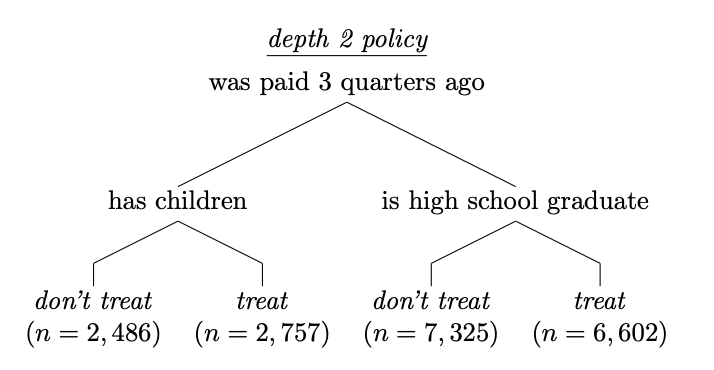
\includegraphics[width=\textwidth]{decision_tree.png}
\end{figure}
\end{frame}

\begin{frame}{Пример: COVID-19 и запрет выхода на улицу для пенсионеров}
Придумайте сами
\end{frame}

% \begin{frame}{Как мы уже говорили, все тут о гетерогенности}
    
% \end{frame}


% \section{Гетерогенность тут!}


% \begin{frame}{Оценка гетерогенности как таковой}
% credit scoring
% \end{frame}

% \begin{frame}{???}
    
% \end{frame}

% \begin{frame}{HTE and CATE}
    
% \end{frame}

% \begin{frame}{trees and honest trees}
    
% \end{frame}

% \begin{frame}{moment conditions GMM/M-estimator}
    
% \end{frame}

% \begin{frame}{Policy learning}
    
% \end{frame}

% \begin{frame}{Pruning trees}
%     fairness etc
% \end{frame}

% \begin{frame}{Custom loss and applications}
    
% \end{frame}

% \begin{frame}{Estimating KDE}
    
% \end{frame}


\end{document}
